\newpage

\section{Introduction}
\label{sec:introduction}

% state the learning objective 
The objective of this laboratory assignment is to study a circuit containing a
sinusoidal voltage source $V_S$ connected to seven resistors, $R$, a dependent voltage source, $V_d$, a dependent current source $I_b$ and a capacitor $C$. The circuit can be seen in Figure~\ref{fig:rc}.


In Section~\ref{sec:analysis}, a theoretical analysis of the circuit is
presented. In Section~\ref{sec:simulation}, the circuit is analysed by
simulation, and the results are compared to the theoretical results obtained in
Section~\ref{sec:analysis}. The conclusions of this study are outlined in
Section~\ref{sec:conclusion}.

\begin{figure}[h] \centering
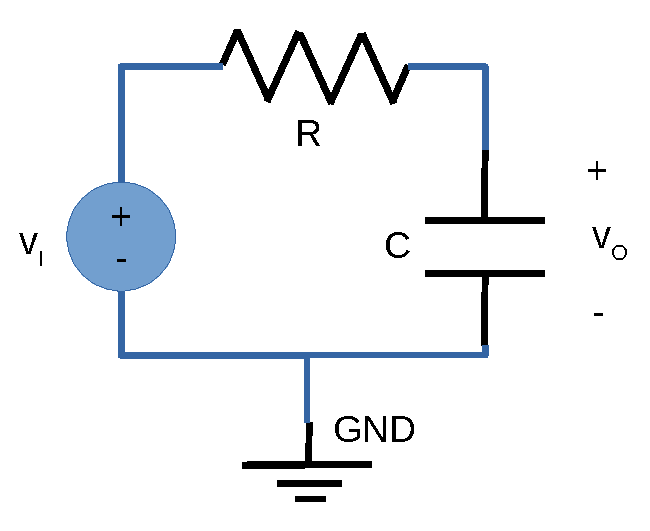
\includegraphics[width=0.7\linewidth]{rc.pdf}
\caption{Given circuit.}
\label{fig:rc}
\end{figure}


